\documentclass[10pt,a4paper]{article}

\usepackage[utf8]{inputenc}
\usepackage{amsmath}
\usepackage{amsfonts}
\usepackage{amssymb}
\usepackage{fullpage}
\usepackage{svg}
\usepackage{titling}
\usepackage{tikz}
\usepackage{physics}
\usepackage{booktabs}
\usepackage{xcolor}
\usepackage{multicol}

\AtBeginDocument{\setlength\abovedisplayskip{12pt}}
\AtBeginDocument{\setlength\belowdisplayskip{12pt}}

\title{NV-Center in Diamond as a Qubit Platform}
\author{Alexander Heilman}

\setlength{\droptitle}{-8em}   % This is your set screw
%\setlength{\parindent}{0pt}

\newenvironment{boxed2}
    {\begin{center}
    \begin{tabular}{|p{0.455\textwidth}|}
    \hline\\
    }
    { 
    \\\\\hline
    \end{tabular} 
    \end{center}
    }

\begin{document}

\vspace{-3cm}
 
\maketitle

\begin{multicols}{2}

\section*{Introduction \& Overview}
Below, we cover the basic usage of NV-Centers in diamond as a qubit platform. We'll first give an overview of the criteria sought in any qubit platform, then describe the NV defect itself and it's relevant energy levels, and then discuss a subset of the criteria applied to the defect. Finally, we'll give a shallow discussion of the modern state of experiment.


\section{Criteria for Qubit Platforms}
Any physical system which we consider as a prospective qubit platform must satisfy a minimal set of criteria. A common set are the so-called 'DiVincenzo Criteria'.


\begin{boxed2}
\vspace{-.4cm}

\textbf{DiVincenzo's Criteria:} David DiVincenzo was a theoretician working on quantum computers in the early 2000's. Through his experience, he delineated 7 criteria which should be sought in prospective qubit platforms \cite{DiVincenzo_2000}.

\medskip

The first five are for quantum computers:


$\bullet$ Scalable with distinguishable states


$\bullet$ Fiduciary initial state

$\bullet$ Long decoherence time


$\bullet$ Universal gate set

$\bullet$ Measureable in some basis

\medskip

And the last two are for quantum networks:


$\bullet$ Transfer from memory to computation

$\bullet$ Faithful transmission across network

\vspace{-.4cm}
\end{boxed2}
Here, we'll focus on three important aspects of any physical realization of a qubit: initialization, control of the states, and the measurement of these states.

First, however, we'll give a brief answer to why we choose defects in diamond as a platform. After, we give an overview of the defect itself and discuss the origin of the relevant energy levels.
Then, we'll discuss how a restricted set of DiVincenzo's criteria are manifestly satisfied in a certain scheme utilizing the NV-Center's spin state as a qubit.

\subsubsection*{Why a Defect?}
Solid state defects offer unique systems that allow us to realize localized electronic states within crystals.

Note then that the defect considered here is chosen primarily because of it's nice energy levels, and a particular asymmetry in an excited state relaxation. The treatment would otherwise apply equally well to most similar systems. 

\subsubsection*{Why Diamond?}
Diamond is then a particularly well suited host material for the defect because of it's low density of phonon modes, and correspondingly high Debye temperature. This lower density of phonon modes generally increases the coherence time of the quantum state of the defect's electrons; allowing us to have a qubit platform that can reach coherence times on the order of seconds to minutes even at room temperature!


\section{NV-Center in Diamond}
An NV-Center in diamond is a pair of neighboring point defects: one being a Nitrogen substitution; and the other being a vacancy, located at one of the nearest neighbor sites of the substitution.

\begin{center}

\includegraphics[scale=0.53]{diamond_nv.pdf}

\end{center}
These defects are well-studied both theoretically and experimentally.


\subsection{Point Group Symmetry}
The center has a $C_{3v}$ site symmetry about the axis connecting the two defects (hereafter referred to as the symmetry axis; we also choose a coordinate system in which this corresponds to the $z$-axis).

\begin{center}
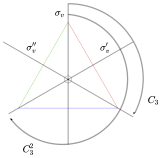
\includegraphics[scale=0.4]{symmetry.pdf}
\end{center}

The $C_{3v}$ symmetry group consists of six group operations. One being the identity identity; two more being rotations of $2\pi/3$ and $4\pi/3$ (often termed $C_3$ and $C_3^2$); and three plane inversions $\sigma_v$, $\sigma_v'$, and $\sigma_v''$. 
Note that these operations have two underlying group generators: $C_3$ and $\sigma_v$. 

$C_{3v}$ symmetry is somewhat common in molecules with a typical example being ammonia ($NH_3$).

\subsection{Charge States}
The bare defect (with the usual valence shells of the neighboring atoms) contains five electrons: three  dangling from the Carbons neighboring the vacancy, and two from the neighboring Nitrogen.

Like many defects (and atomic/molecular systems for that matter), the NV-Center can then hold one of a few charge states. The most common being: neutral (all local atoms have exactly their valence electrons), and negative (-, with an extra electron, filling the neighboring Carbons' valence shell).

If a resource doesn't make specific reference to the charge state of the NV defect, it's likely referring to the negative charge state (with an extra electron localized to the defect). This is also the charge state which we will treat exclusively here.

\subsection{Spin States}
For the pair of electrons localized to the negatively charged defect, the spin state can either be in a singlet or triplet state. 

In the triplet state, there is a total spin of either $s=1,0$ or $-1$, each with a corresponding range of allowed magnetic quantum number $m_s=-J,-J+1,...,J$ (here we take this to denote the projection of the spin along the $z$-axis).
The singlet state then has total spin of $J=0$ and a corresponding magnetic quantum number $m_s=0$.

\subsection{Spin Hamiltonian}
We wish to use the spin state of the electron pair (in the electronic ground state) as our qubit state. As such, we need consider the relevant effects that influence the energy level of the spin state.

Spins generally interact most strongly with magnetic fields and other spins (which effectively generate magnetic fields). These different influences are broken up into corresponding effects, which we cover and discuss independently below.

\subsubsection{Zero-Field Splitting}
Zero-field splitting (ZFS) refers to the electron-electron interaction (between their spins) of the pair. With no other magnetic fields around, or other spins, this will result in a splitting of the $m_s$ energy levels dependent only on the magnitude (so that $m_s=+1,-1$ are still degenerate). Generally, these interactions can be described via a term as below:
$$
H_{ZFS}=\vec{\hat{S}}\mathbf{D}\vec{\hat{S}}
$$
where $\vec{\hat{S}}$ is the spin state of the pair, and $\mathbf{D}$ is the dipole-dipole interaction tensor (which is necessarily symmetric and traceless). 

In the case of a singlet state, there is only one state, and hence the ZFS is irrelevant. However, for the triplet state, the relevant term may be expanded as below (where we choose a basis that diagonalizes the interaction tensor).
$$
H_{ZFS}=D \Big( S_z^2-\frac{1}{3}S(S+1)\Big) + E (S_x^2-S_y^2) 
$$
where $D=\frac{3}{2}D_{zz}$ and $E=\frac{1}{2}(D_{xx}-D_{yy})$. Further assuming the wavefunction of the defect state to be symmetric under rotation about the $z$-axis (which we've chosen to align with the symmetry axis of the defect, connecting the vacancy and the substitution), we may further take $E=0$ in this case.

\subsubsection{Quadrapole Interactions}
The quadrapole interaction refers to the self interaction of the nitrogen nuclei's spin. 
$$
H_{Quad}=\vec{\hat{I}}_N\mathbf{Q} \vec{\hat{I}}_N
$$
where $\vec{\hat{I}}_N$ refers to the nuclear spin vector of the Nitrogen atom, and $\mathbf{Q}$ refers to the corresponding quadrapole interaction tensor.

\subsubsection{Fine Structure}
The fine structure generally refers to the spin-orbit coupling of the electrons in their orbitals, and hence can be modeled as a term of the form below:
$$
H_{SOC}\propto \vec{\hat{S}}\cdot \vec{\hat{L}}
$$ 
where now $\vec{\hat{L}}$ is the orbital angular momentum of the spin in it's orbital. 

For the triplet ground state of the system ($^3A_2$), the effective orbital angular momentum of the electron is zero, and hence this term is negligible in the following considerations \cite{gali2019ab} for our choice of computational basis.

\subsubsection{Hyperfine Interactions}
Hyperfine interactions refer to the spin-spin interactions between the electron pair and the neighboring nuclei, including the local Nitrogen and the surrounding Carbon.
$$
H_{Hyperfine}=\vec{\hat{S}}\big(\mathbf{A}_N\vec{\hat{I_N}}+\sum_i\mathbf{A}_{C_i}\vec{\hat{I}}_{C_i}\big)
$$
where $\vec{\hat{I}}_{C_i}$ denotes the nuclear spin vector of the $i$-th Carbon atom, and $\mathbf{A}_j$ denotes the hyperfine interaction tensor for the $j$-th atom. 

\subsubsection{Zeeman Effect}
The Zeeman effect refers to the splitting of spin-state energy levels aligned or anti-aligned with an external field.
$$
H_{Zeeman}=\big(\vec{\hat{S}}\mathbf{g}_s+\vec{\hat{I}}_N\mathbf{g}_N+\sum_i\vec{\hat{I}}_{C_i}\mathbf{g}_{C_i}\big)\vec{B}
$$
where $\vec{B}$ denotes the externally applied magnetic field vector and $\mathbf{g}$ denotes the Zeeman interaction tensor (which is closely related to the gyromagnetic ratios of the corresponding element).

\subsubsection{Stark Effect}
For an externally applied electric field, there also are some corresponding effects on the energy levels of the system. This is generally referred to as the Stark effect. Here we will completeley disregard any influence of external electric field (as they tend to be less impactful than the magnetic influences on spin states energy levels).

It should be noted that the influence of strain on the system generally can be modeled as an external electric field acting on the system.

\subsubsection{Simplifications}
While the many interactions covered above are relevant in modern research of the defect, we wish only to portray the system as clearly as possible as a potential qubit. In this sense, we will simplify the relevant Hamiltonian immensely and consider only a few of the above effects, resulting in the following effective spin Hamiltonian (following that used in \cite{PhysRevLett.129.100501}):
$$
H_{\text{eff}} = DS_z^2 + \omega_eS_z + QI_z^2 +\omega_nI_z + AS_zI_z
$$
The relevant coupling constants have been determined to be the following:
$D=2\pi\times (2.87 GHz)$, the dipole coupling constant;
$Q=2\pi\times (-4.95 GHz)$, the nuclear quadrapole coupling constant;
$A=2\pi\times (-2.16 GHz)$, the hyperfine coupling constant.

In the following, we will generally assume $I_z$ to be fixed, so that it results primarily in an overall shift of all of the energy states. Furthermore, we will assume that the Zeeman splitting is substantially larger than the hyperfine interaction $AS_zI_z$ so that we may effectively neglect it's effect as well (though it's inclusion doesn't at all affect the following discussion since it only acts to lift the degeneracy of the different $m_s$ states).

Essentially, we just need a set of quantum states that are discernible (with different energy levels) that we then can read out by some means and control. The 

\subsection{Energy States}
The relevant energy states of the NV-Center are then those depicted below.
\begin{center}
\includegraphics[scale=0.72]{energy_raw_inline.pdf}
\end{center}
The common notation has $^3A_1$ denoting the triplet's electronic ground state, $^3E$ denoting the triplet's first excited state, $^1A_2$ denoting the singlet's ground state, and $^1 E$ denoting the singlet's first excited state.

Note that the $m_s=\pm 1$ states are degenerate (with our simplifications) in the absence of any external magnetic field.

\section{NV-Center as a Qubit Platform}
We now will consider how we may utilize these spin states as a qubit platform.
We first need to choose two energy levels for use as our qubit states. The prototypical choice is the triplet ground state's $m_s=0$ level as the $\vert 0 \rangle$ state of the computational basis and the triplet ground state's $m_s=-1$ level as the computational basis' $\vert 1 \rangle$ state.
\begin{center}
\includegraphics[scale=1.05]{energy_qubit.pdf}
\end{center} 
Of course, this requires some externally applied magnetic field that allows the degeneracy of the two non-zero $m_s$ states to be lifted. Typically, this is applied at a magnitude such that the transition between the newly defined $\vert 0 \rangle$ and $\vert 1 \rangle$ states corresponds to the microwave regime.

With these computational basis states now associated with some real quantum states, we will consider three basic elements of any quantum computer: initialization, control, and measurement.

\subsection{Initialization}
Initialization to the zero state can be achieved by an asymmetric relaxation from the first excited triplet state ($^3E$) to the triplet ground state ($^3A$). 

First applying a resonant pulse (532 nm) excites all triplet ground states to their corresponding excited states ($\Delta m_s=0$).
\begin{center}
\includegraphics[scale=0.5]{energy_init_relax.pdf}
\end{center}
Excited $m_s=0$ states then have been shown to decay back into $m_s=0$ ground states via another optical transition, but $m_s=\pm 1$ excited states allow a non-radiative (vibronic; mediated by phonons as well as photons) decay mode via the singlet states, back into the $m_s=0$ ground state. 

This may be exploited to intialize the spin state into our $\vert 0 \rangle$ state. Since the transitions generally increase the population of the $\vert 0 \rangle$ state and decrease the population of the $\vert 1 \rangle$ state, the state can be considered to be initialized if the resonant pulses are applied enough times.



\subsection{Measurement}
Much like the initialization technique, optically detected magnetic resonance (ODMR) takes advantage of the asymmetric relaxation modes of the excited state.

The asymmetric relaxation of the spin states allows us to determine the final (observed/measured) state of the system by essentially hitting the state with another resonant pulse (of the wavelength corresponding to the first excitation of the electronic state) and seeing if we observe another optical transition back down.
\begin{center}
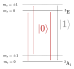
\includegraphics[scale=0.76]{energy_measure.pdf}
\end{center}
Hence, if the defect flouresces when hit with a resonant pulse, it was measured to be in the $\vert 0 \rangle$ state, but if it's 'dark' after a resonant pulse, it can be considered to have been in the $\vert 1 \rangle$ state.

Note that the similarity in mechanism allows our read-out to essentially be part of the next computation's initialization.


One problem, however, is the possibility of internal reflection of the emitted photon. This can be solved with an immersion lens built into the diamond \cite{hadden2010strongly}.

\subsection{Control}
With a known initial state and a means to measure the resulting state, we now need some way to control the system. 

Microwave pulses with polarization perpendicular to the symmetry axis can be used to induce Rabi oscillations between the $\vert 0 \rangle$ and $\vert 1 \rangle$ states. 

Using such a technique, we provide an example data set (with resulting fluorescence indicative of the state via ODMR plotted on the y-axis) from \cite{PhysRevLett.105.177403} below.

\begin{center}
\includegraphics[scale=1]{rabi.png}
\end{center}
While this gives a visual understanding of the phenomena, a more in-depth treatment requires consideration of a rotating frame Hamiltonian with a new term accounting for the resonant microwave magnetic field (much as in nuclear magnetic resonance). For an overview of such a frame, see \cite{PhysRevB.84.161403}.


\section{Conclusion \& Outlook}
Here, we've given an intuitive overview of the basics of the NV-Center and a simple means by which we may realize the system as a qubit. In actuality, we need a scalable system with an arbitrary number of qubits that can somehow interact with each other. This is generally achieved in two ways: by using the NV-center as a register to read out the surrounding the nuclear spins (via the hyperfine interactions); and by coupling photons to the quantum states of distant centers, so that the distant centers may interact via their coupled photons. 

Recently, 10-qubit control was performed using the center's spin state and the surrounding nuclear spins \cite{PhysRevX.9.031045}.
Spin-photon entanglement has also been demonstrated and used to have distant centers interact up to a distance of 1.3 km \cite{nemoto2016photonic}.


Regardless, this is a promising candidate due in large part to it's stability (relatively long decoherence times) even at room temperature.

For a more in-depth introduction and (somewhat outdated) overview of the experimental progress in the technique, see
\cite{childress2013diamond}.
\end{multicols}

\nocite{*}

\bibliographystyle{plain}

\bibliography{nv} 

\end{document}
